\documentclass[12pt]{article}
% \usepackage[top=1in,left=1in, right = 1in, footskip=1in]{geometry}
\usepackage[top=1in,footskip=1in]{geometry}

\usepackage{graphicx}
\usepackage{xspace}
%\usepackage{adjustbox}

\usepackage{pdflscape}

\usepackage{grffile}

\newcommand{\comment}{\showcomment}
%% \newcommand{\comment}{\nocomment}

\newcommand{\showcomment}[3]{\textcolor{#1}{\textbf{[#2: }\textsl{#3}\textbf{]}}}
\newcommand{\nocomment}[3]{}

\newcommand{\jd}[1]{\comment{cyan}{JD}{#1}}
\newcommand{\swp}[1]{\comment{magenta}{SWP}{#1}}
\newcommand{\bmb}[1]{\comment{blue}{BMB}{#1}}
\newcommand{\djde}[1]{\comment{red}{DJDE}{#1}}

\newcommand{\eref}[1]{Eq.~(\ref{eq:#1})}
\newcommand{\fref}[1]{Fig.~\ref{fig:#1}}
\newcommand{\Fref}[1]{Fig.~\ref{fig:#1}}
\newcommand{\sref}[1]{Sec.~\ref{#1}}
\newcommand{\frange}[2]{Fig.~\ref{fig:#1}--\ref{fig:#2}}
\newcommand{\tref}[1]{Table~\ref{tab:#1}}
\newcommand{\tlab}[1]{\label{tab:#1}}
\newcommand{\seminar}{SE\mbox{$^m$}I\mbox{$^n$}R}

\usepackage{amsthm}
\usepackage{amsmath}
\usepackage{amssymb}
\usepackage{amsfonts}
\usepackage[utf8]{inputenc} % make sure fancy dashes etc. don't get dropped

\usepackage{lineno}
\linenumbers

\usepackage[pdfencoding=auto, psdextra]{hyperref}

\usepackage{natbib}
\bibliographystyle{chicago}
\date{\today}

\usepackage{xspace}
\newcommand*{\ie}{i.e.\@\xspace}

\usepackage{color}

\newcommand{\Rx}[1]{\ensuremath{{\mathcal R}_{#1}}\xspace} 
\newcommand{\RR}{\ensuremath{{\mathcal R}}\xspace}
\newcommand{\Rres}{\Rx{\mathrm{res}}}
\newcommand{\Rinv}{\Rx{\mathrm{inv}}}
\newcommand{\Rhat}{\ensuremath{{\hat\RR}}}
\newcommand{\Rt}{\ensuremath{{\mathcal R}(t)}\xspace}
\newcommand{\tsub}[2]{#1_{{\textrm{\tiny #2}}}}
\newcommand{\dd}[1]{\ensuremath{\, \mathrm{d}#1}}
\newcommand{\dtau}{\dd{\tau}}
\newcommand{\dx}{\dd{x}}
\newcommand{\dsigma}{\dd{\sigma}}

\newcommand{\rx}[1]{\ensuremath{{r}_{#1}}\xspace} 
\newcommand{\rres}{\rx{\mathrm{res}}}
\newcommand{\rinv}{\rx{\mathrm{inv}}}

\newcommand{\psymp}{\ensuremath{p}} %% primary symptom time
\newcommand{\ssymp}{\ensuremath{s}} %% secondary symptom time
\newcommand{\pinf}{\ensuremath{\alpha_1}} %% primary infection time
\newcommand{\sinf}{\ensuremath{\alpha_2}} %% secondary infection time

\newcommand{\psize}{{\mathcal P}} %% primary cohort size
\newcommand{\ssize}{{\mathcal S}} %% secondary cohort size

\newcommand{\gtime}{\tau_{\rm g}} %% generation interval
\newcommand{\gdist}{g} %% generation-interval distribution
\newcommand{\idist}{\ell} %% incubation-period distribution

\newcommand{\total}{{\mathcal T}} %% total number of serial intervals

\usepackage{lettrine}

\newcommand{\dropcapfont}{\fontfamily{lmss}\bfseries\fontsize{26pt}{28pt}\selectfont}
\newcommand{\dropcap}[1]{\lettrine[lines=2,lraise=0.05,findent=0.1em, nindent=0em]{{\dropcapfont{#1}}}{}}

\begin{document}

\begin{flushleft}{
	\Large
	\textbf\newline{
	  Strategic coexistence theory for evolutionary games
	}
}
\newline
\\
Sang Woo Park\textsuperscript{1,2,*}
\\
\bigskip
\textbf{1} School of Biological Sciences, Seoul National University, Seoul, Korea\\
\textbf{2} Institute for Data Innovation in Science, Seoul National University, Seoul, Korea
*Corresponding author: sangwoopark@snu.ac.kr
\end{flushleft}

\section*{Abstract}

Evolutionary game theory and ecological coexistence theory both seek to predict the outcome of competition between biological entities, be they strategies or species, but the two fields have relied on largely separate approaches. 
Replicator equations provide a foundation for predicting the outcome of strategic competition, but comparing how different mechanisms alter competition across games remains challenging. 
Inspired by modern coexistence theory from community ecology, we develop Strategic Coexistence Theory (SCT), which translates payoff-based invasion conditions at monomorphic boundary conditions into strategic niche differences and fitness differences between any two competing strategies described by classic replicator dynamics.
We show that SCT recovers the classic classification of two-strategy games and also allows us to compare mechanisms for the evolution of cooperation from different games on the shared niche-fitness difference space.
In stochastic games, environmental stochasticity increases both boundary invasion growth rates, whereas in multiplayer public-goods games, nonlinear benefits can either stabilize or destabilize competition. 
These applications also show that the number or stability of internal equilibria generally cannot be predicted from invasion growth rates at monomorphic boundaries, illustrating a key limitation of characterizing competitive systems using boundary invasion rates alone.
Together, these results show that SCT provides a coexistence-theoretic perspective for characterizing how different mechanisms alter strategy competition across games.

\section*{Significance statement}

Evolutionary game theory provides a powerful framework for predicting the outcome of competition between strategies.
However, comparing how different mechanisms contribute to different outcomes across games remains challenging. 
Motivated by Modern Coexistence Theory from community ecology, we developed Strategic Coexistence Theory (SCT), which decomposes invasion rates of strategies when rare into strategic niche and fitness differences. 
Applications to classic games, mechanisms of cooperation, environmental stochasticity, and multiplayer public-goods games place diverse models onto shared axes of niche and fitness differences.
These applications also point to a limitation to predicting coexistence from mutual invasion conditions at the boundary.
This approach links ecological theory with replicator dynamics, providing a common language for comparing strategy competition across games.

\section*{Introduction}

Understanding the mechanisms that promote the evolutionary stability of competing strategies is a fundamental aim in evolutionary biology \citep{lewontin1961evolution,slobodkin1964strategy,smith1973logic,taylor1978evolutionary}.
To this end, evolutionary game theory (EGT) and replicator dynamics have provided key foundations, allowing us to predict the outcome of strategic competition through payoff inequalities, invasion criteria, and stability analysis \citep{schuster1983replicator,hofbauer1998evolutionary,cressman2003evolutionary,cressman2014replicator}.
Recently, there has been growing interest in characterizing similarities between replicator dynamics and the dynamics of competing species \citep{gokhale2025higher,tarnita2025reconciling,allesina2026global}, building on the classical mathematical equivalence between replicator equations and generalized Lotka–Volterra models \citep{hofbauer1981occurrence,page2002unifying}.
In particular, \cite{tarnita2025reconciling} argued that EGT approaches for studying complex interactions may inform analyses of analogous ecological interactions, such as higher order and hierarchical interactions.
Building on this renewed connection between ecological and evolutionary dynamics, we suggest that interpreting evolutionary games from the ecological perspective of strategy coexistence may enable comparisons of mechanisms in different games within a common framework.

Interestingly, even a simple two-strategy game can yield heterogeneous outcomes that mirror those in community ecology \citep{hauert2002effects,szabo2007evolutionary,cooney2020analysis,tarnita2025reconciling}: the dominance of a single strategy (prisoner’s dilemma and harmony games), coexistence (hawk–dove games), and bistability (stag-hunt games).
Such differences in conditions that promote evolutionary stability and dominance of a single strategy and those that permit strategy coexistence indicate that EGT can be understood from the perspective of coexistence theory \citep{motro1991co,doebeli2004evolutionary,hauert2004spatial,doebeli2005models,gore2009snowdrift,souza2009evolution,archetti2011coexistence,steidinger2014coexistence,tarnita2025reconciling}.
In fact, stable polymorphisms of evolutionary strategies are observed in microbial and other biological systems \citep{gore2009snowdrift,cordero2012public,kocher2018genetic,pollak2021public,lin2024interspecific}, but a coexistence-theoretic perspective has often remained implicit.
Recasting game dynamics as a coexistence problem immediately raises the following question: when two strategies coexist, does the corresponding mechanism stabilize or equalize competition \citep{chesson2000mechanisms}?
While EGT allows us to predict whether two strategies can coexist or not, a common framework for comparing how different mechanisms stabilize or equalize competition across different games remains elusive.

Modern coexistence theory (MCT) from community ecology presents a particularly useful framework for quantifying coexistence mechanisms \citep{chesson2000mechanisms,adler2007niche,godoy2014phylogenetic,godoy2014phenology,kraft2015plant,adler2026have}. 
MCT predicts that coexistence of two competing entities, be they species or strategies, requires stabilizing niche differences to overcome average fitness differences \citep{chesson2000mechanisms,adler2007niche,kraft2015plant}.
In community ecology, stabilizing niche differences represent differences in factors that limit the growth of competing species, causing each species to limit itself more than it limits its competitor \citep{chesson2000mechanisms}.
In EGT, a strategy’s niche can be interpreted as strategic environments defined by the composition of competing strategies and the resulting interactions \citep{taylor1978evolutionary,cressman2014replicator,tarnita2025reconciling}.
From the perspective of MCT, stabilizing niche differences arise when each strategy is favored under the monomorphic boundary condition created by its competitor than under the one created by itself, such that the spread of each strategy limits its own relative growth and favors the recovery of its competitor.
In contrast, fitness differences represent differences in the ability of each entity to compete under the limiting environments created by its competitor \citep{chesson2000mechanisms}.
This differs from payoff differences in EGT, which depend on the underlying strategy frequency and therefore combine both stabilizing effects caused by changes in the strategic environment and residual fitness differences that favor one strategy over another \citep{taylor1978evolutionary,cressman2014replicator,tarnita2025reconciling}.

So far, MCT has been primarily utilized for understanding species coexistence, but recent work showed that analogous framework can be derived for other biological systems, especially for studying pathogen strain competition, allowing one to directly quantify niche and fitness differences of competing entities, be they species or strains \citep{sieben2022quantifying,park2024predicting,park2026unifying}.
Inspired by this effort, we present Strategic Coexistence Theory (SCT), which translates the invasion growth rates of competing strategies at monomorphic boundary conditions into strategic niche and fitness differences.
In doing so, we apply SCT to four different case studies: classic two-strategy games, mechanisms for the evolution of cooperation, environmental stochasticity, and multiplayer public-goods games.
For classic-game and stochasticity applications, we consider four different game types: Prisoner’s Dilemma, Hawk–Dove, Stag–Hunt, and Harmony.
In the cooperation-mechanism application, prisoner's dilemma serves as a common baseline for comparing five pairwise mechanisms.
In contrast, the multiplayer public-goods application considers an explicit $N$-player game with nonlinearity effect on public goods.

Overall, these examples illustrate the utility of a coexistence-theoretic perspective for comparing mechanisms of strategy competition.
However, since SCT is based on invasion growth rates at monomorphic boundary conditions, it does not provide a complete picture for the interior dynamics.
Within this scope, SCT provides a common framework for linking coexistence theory in community ecology with evolutionary game theory.

\section*{Strategic coexistence theory}

Here, we present a brief derivation of strategic coexistence theory (SCT) (Figure 1).
To do so, we begin with a classic replicator equation, which allows us to model changes in the frequency of competing strategies based on their payoffs \citep{schuster1983replicator,hofbauer1998evolutionary,cressman2003evolutionary,cressman2014replicator}:
\begin{equation}
\frac{dx_i}{dt} = x_i (\pi_i(\mathbf{x}) - \bar{\pi}(\mathbf{x})),
\end{equation}
where $x_i$ represents the frequency of strategy $i$, $\pi_i(\mathbf{x})$ represents the payoff of strategy $i$ for a given strategy distribution $\mathbf{x}$, and $\bar{\pi}(\mathbf{x}) = \sum_i \pi_i(\mathbf{x}) x_i$ represents the average payoff. Since strategy frequencies must sum to 1 (i.e., $\sum_i x_i = 1$), a single-strategy equilibrium dominated by strategy $i$ can be described by a unit vector $\mathbf{e}_i$, where all elements are equal to zero except for the $i$-th element. 
We use these single-strategy equilibria to define niche and fitness differences between two competing strategies $i$ and $j$.

Because payoffs in many games can be negative, payoff ratios can be difficult to interpret.
Thus, we work on a positive multiplicative scale by exponentiating the payoff terms:
\begin{equation}
W_i(\mathbf{x}) = \exp(\pi_i(\mathbf{x})).
\end{equation}
This exponential transformation is convenient because it preserves the payoff ordering and does not alter the invasion conditions.
Therefore, this allows us to compare strategic environments through ratios, as in modern coexistence theory.
For convenience, we refer to $W_i(\mathbf{x})$ as the multiplicative payoff of strategy $i$.

\begin{figure}[!th]
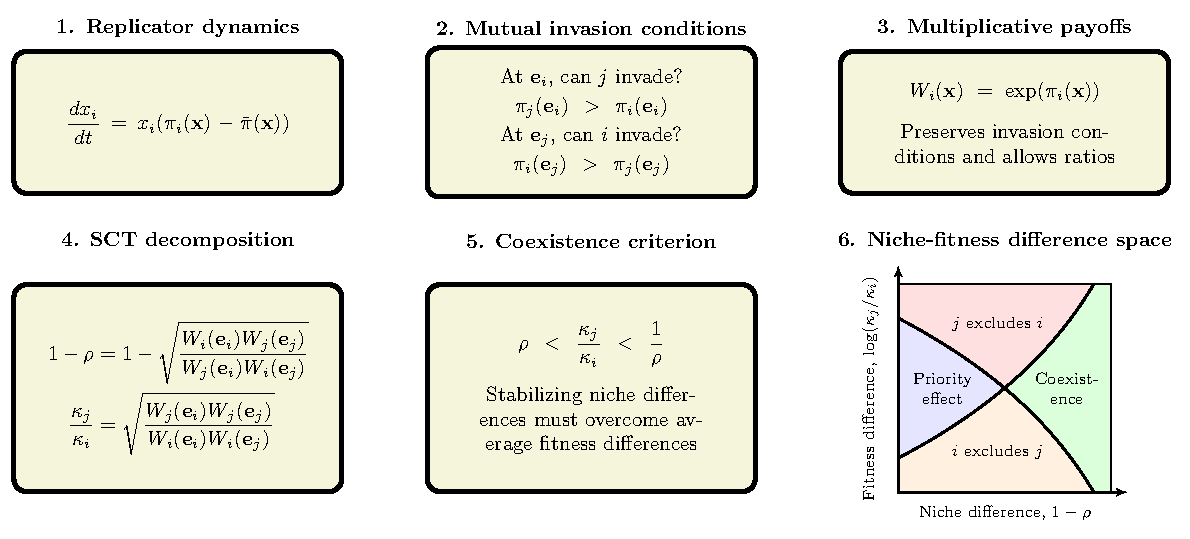
\includegraphics[width=\textwidth]{../diagram_sct/diagram_sct.pdf}
\caption{
\textbf{A schematic diagram summarizing strategic coexistence theory.}
Strategic coexistence theory decomposes pairwise replicator dynamics into stabilizing and equalizing mechanisms.
Mutual invasion conditions can be rewritten on a multiplicative payoff scale, allowing us to derive strategic niche difference $1-\rho$ and fitness difference $\kappa_j/\kappa_i$ based on multiplicative payoff ratios.
Then, the inequality $\rho < \kappa_j/\kappa_i < 1/\rho$ determines mutual invasion.
We note that the exact values of niche and fitness differences are sensitive to payoff scaling, while dynamical outcomes are still preserved. 
}
\end{figure}

First, we define the niche overlap $\rho$ between strategies $i$ and $j$ as the ratio between the geometric mean of each strategy’s multiplicative payoff in the strategic environment that it creates when common, $\sqrt{W_i(\mathbf{e}_i) W_j(\mathbf{e}_j)}$, and the geometric mean of each strategy’s multiplicative payoff in the environment generated by its competitor, $\sqrt{W_j(\mathbf{e}_i) W_i(\mathbf{e}_j)}$. 
The corresponding niche difference is then given by
\begin{equation}
1- \rho = 1-\sqrt{\frac{W_i(\mathbf{e}_i) W_j(\mathbf{e}_j)}{W_j(\mathbf{e}_i) W_i(\mathbf{e}_j)}}.
\end{equation}
When $1-\rho > 0$, the geometric mean of the multiplicative payoffs across the two strategies is greater in competitor-generated monomorphic environments than in self-generated monomorphic environments.
In other words, intraspecific competition is stronger than interspecific competition at the boundary.
When $\rho>1$, we interpret the resulting negative niche difference, $1-\rho<0$, as a destabilizing effect corresponding to positive frequency dependence, meaning that the strategy that is already common is favored.

Second, we define the fitness difference as the ratio between the geometric means of the multiplicative payoff of each strategy across the two single-strategy environments:
\begin{equation}
\frac{\kappa_j}{\kappa_i} = \sqrt{\frac{W_j(\mathbf{e}_i)W_j(\mathbf{e}_j)}{W_i(\mathbf{e}_i) W_i(\mathbf{e}_j)}}.
\end{equation}
In other words, strategy $j$ has an average competitive advantage over strategy $i$ ($\kappa_j/\kappa_i > 1$) when it performs better, on average, across the environments generated by itself and its competitor.

We note that niche and fitness difference can be equivalently written in terms of the invasion growth rates at the monomorphic boundary conditions:
\begin{align}
1- \rho &= 1 - \exp\left(-\frac{r_{i|j} + r_{j|i}}{2} \right),\\
\frac{\kappa_j}{\kappa_i} &= \exp\left(\frac{r_{j|i} - r_{i|j}}{2}\right),
\end{align}
where $r_{i|j} = \pi_i(\mathbf{e}_j) - \pi_j(\mathbf{e}_j)$ and $r_{j|i} = \pi_j(\mathbf{e}_i) - \pi_i(\mathbf{e}_i)$ represent the growth rate of strategy $i$ and $j$ when strategy $j$ and $i$ are at monomorphic equilibrium, respectively.
These growth rates also correspond to payoff differences.
This parameterization is particularly useful because it allows us to compute niche and fitness differences even when the selection gradient governing replicator dynamics do not uniquely separate into two payoff values.

Together, for any two strategies described by the classic replicator equation, mutual invasion requires stabilizing niche differences to overcome average fitness differences.
Specifically, the condition for mutual invasion can be rewritten as \citep{chesson2000mechanisms}:
\begin{equation}
\rho < \frac{\kappa_j}{\kappa_i} < \frac{1}{\rho}.
\end{equation}
In simple systems with monotonic interior dynamics, these boundary invasion conditions also determine the global dynamical outcome, allowing competition to be classified into coexistence, competitive-exclusion, and priority-effect regimes.
However, MCT and SCT are based on invasion conditions at the boundaries and do not generally characterize nonlinear interior dynamics.
Mutual invasion still guarantees at least one stable internal equilibrium, but it does not determine the number or stability of additional internal equilibria. 
Likewise, boundary conditions associated with competitive exclusion or priority effects do not rule out stable internal equilibria.
As we show later, nonlinear dynamics can allow stable coexistence even when a system lies in the boundary-defined competitive-exclusion regime. 
Therefore, when interior dynamics are nonmonotonic, we use these classifications to describe boundary invasibility rather than complete dynamical outcomes.

Despite this limitation, the mutual-invasion inequality provides a useful perspective for comparing how different mechanisms alter boundary invasibility.
Notably, the inequality can be applied to any pairwise comparison between two strategies described by the classic replicator equation because $\rho$ and $\kappa_j/\kappa_i$ can be calculated directly from ratios of multiplicative payoffs.
This provides a common framework for comparing qualitative changes in boundary invasibility across different games.
Detailed derivations are provided in Supplementary Text S1.

We note that the absolute magnitudes of niche and fitness differences are sensitive to payoff scaling because they are defined on an exponentiated payoff scale.
Therefore, while SCT allows us to compare different games on shared axes, we cannot compare the exact values of niche and fitness differences across different games.
Nonetheless, as we show in Supplementary Text S2, the qualitative outcome of strategic competition under SCT is preserved because payoff rescaling preserves payoff orderings.
Therefore, we focus on comparing qualitative outcomes from SCT, including directions of change in niche and fitness difference and resulting dynamical regimes, and refrain from making any comparisons of magnitude of niche and fitness difference values.

\section*{Classic two-strategy games}

As an illustrative example, we begin with classic two-strategy games \citep{hauert2002effects,szabo2007evolutionary,cooney2020analysis,tarnita2025reconciling}, which can be described by the following payoff matrix (Figure 2A):
\begin{equation}
\begin{pmatrix}
R & S \\
T & P
\end{pmatrix}.
\end{equation}
Here, the first and second rows represent strategies 1 and 2, respectively, and the columns represent the strategy of the interacting opponent. 
Writing $x_1$ to denote the frequency of strategy 1, the expected payoffs are
\begin{align}
\pi_1(\mathbf{x}) &= R x_1 + S(1-x_1),\\
\pi_2(\mathbf{x}) &= T x_1 + P(1-x_1).
\end{align}
Thus, the dynamics can be written as
\begin{equation}
\frac{dx_1}{dt} = x_1(1-x_1)\left[(R-T)x_1 + (S-P)(1-x_1)\right].
\end{equation}
The signs of $T-R$ and $S-P$ determine whether each strategy can invade the other when rare.
Specifically, strategy 2 can invade strategy 1 when $T>R$, whereas strategy 1 can invade strategy 2 when $S>P$. 
These two invasion conditions partition the game space into four regimes (Figure 2B): 
prisoner’s dilemma ($T>R > P>S$), hawk--dove game ($T>R$, $S>P$), stag--hunt game ($R>T$, $P>S$), and harmony game ($R>T$, $S>P$).
In standard EGT, these outcomes are obtained by analyzing the stability of equilibrium conditions. 
For simple games, this analysis is straightforward.

\begin{figure}[!ht]
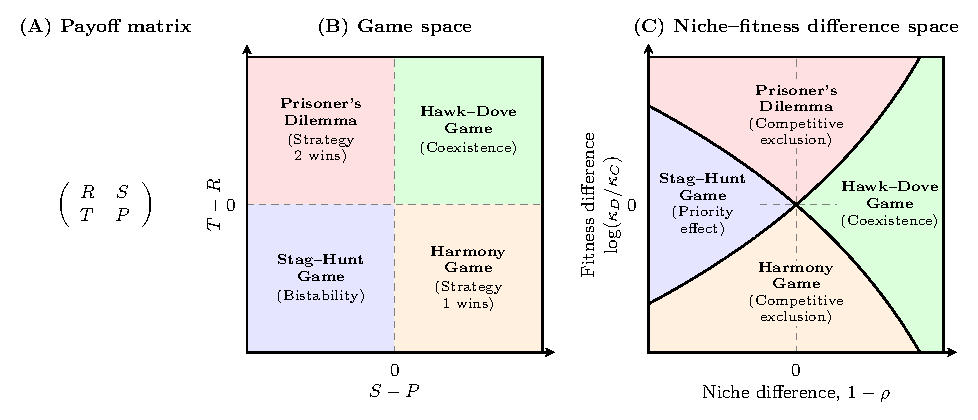
\includegraphics[width=\textwidth]{../diagram_two/diagram_two.pdf}
\caption{
\textbf{Coexistence-theoretic interpretation of classic two-strategy games.}
(A) General payoff matrix for a two-strategy game, where rows represent the focal strategy and columns represent the strategy of the interacting opponent.
(B) Classification of four classic games based on the payoff differences $T-R$ and $S-P$.
Prisoner's dilemma and harmony games lead to the dominance of one strategy;
hawk--dove games allow coexistence;
and stag--hunt games result in bistability.
(C) Mapping of the same four games onto niche--fitness difference space.
Hawk--dove games correspond to the coexistence regime, where stabilizing niche differences overcome fitness differences.
Prisoner's dilemma and harmony games correspond to competitive-exclusion regimes, whereas stag--hunt games correspond to the priority-effect regime.
Negative values of $1-\rho$ indicate positive frequency dependence and destabilization.
$R > P$ is assumed throughout, but this does not affect coexistence outcome in any way.
}
\end{figure}

A coexistence-theoretic approach recovers the same classification (Figure 2C). 
For a two-strategy game determined by this payoff matrix, the niche difference and fitness difference are given by the following set of equations (Supplementary Text S3):
\begin{align}
1- \rho &= 1 - \exp\left(\frac{R + P - S - T}{2}\right),\label{eq:nd}\\
\frac{\kappa_2}{\kappa_1} &= \exp\left(\frac{T+P-R-S}{2}\right)\label{eq:fd}.
\end{align}
As shown above, mutual invasion requires $\rho < \kappa_2/\kappa_1 < 1/\rho$, which is equivalent to $T > R$ and $S > P$.
This corresponds to the hawk--dove game, in which each strategy can invade its competitor when rare and the two strategies coexist. 
The remaining games also have natural interpretations in niche--fitness difference space. 
Prisoner’s dilemma and harmony games represent competitive exclusion regimes, where one strategy has a fitness advantage that exceeds niche differences.
In contrast, stag--hunt games represent a priority-effect regime, where neither strategy can invade the other and the outcome depends on initial conditions.
Therefore, coexistence theory not only allows us to recover the classic results from two-strategy games but also expresses these results in terms of niche and fitness differences.
Building on this, we next apply this framework to comparing core mechanisms of cooperation.

\section*{Comparisons of mechanisms for the evolution of cooperation}

Understanding mechanisms that promote the evolution of cooperation is a central goal in evolutionary biology \citep{west2007evolutionary,fletcher2008simple,clutton2009cooperation,kingma2014group,rakoff2016evolution,hilbe2018evolution,apicella2019evolution,west2021ten,lee2022bacterial,palmer2022bacterial,michel2024evolution}.
Here, we compare five classic mechanisms for the evolution of cooperation using SCT \citep{nowak2006five} and ask how they differ from the perspective of SCT.
Specifically, we consider the following mechanisms: kin selection, direct reciprocity, indirect reciprocity, network reciprocity, and group selection (Figure 3A).
Following \cite{nowak2006five}, these five mechanisms are formulated as modifications of a pairwise Prisoner’s Dilemma.
We use the Prisoner’s Dilemma as a common baseline for comparing these specific formulations in this case study, rather than as a general model of cooperation.

Kin selection favors cooperation when two interacting individuals are genetic relatives, where the genetic relatedness $r$ must be greater than the cost-to-benefit ratio: $r > c/b$ \citep{hamilton1964genetical}.
Direct reciprocity favors cooperation when current cooperation may promote future cooperation by the same individual through repeated encounters \citep{trivers1971evolution,axelrod1981evolution}.
In this case, the probability of repeated interaction (i.e., ``next round'') must be greater than the cost-to-benefit ratio: $w > c/b$.
Indirect reciprocity favors cooperation when current cooperation may promote future cooperation by different individuals through reputation \citep{nowak1998evolution,wedekind2000cooperation,nowak2005evolution}.
Thus, the social acquaintanceship (i.e., the probability of knowing someone’s reputation) must be greater than the cost-to-benefit ratio: $q > c/b$.
Network reciprocity favors cooperation via clustering of cooperators, requiring the benefit-to-cost ratio to be greater than the average number of neighbors: $b/c > k$ \citep{nowak1992evolutionary,lieberman2005evolutionary}.
Finally, group selection favors cooperation via multilevel selection, where groups with more cooperators exhibit faster growth at the group level even if defectors reproduce faster at the individual level \citep{traulsen2006evolution}.
This requires $b/c > 1 + (n/m)$, where $n$ is the maximum group size and $m$ is the number of groups.
All of these mechanisms can be described by a simple $2\times 2$ payoff matrix \citep{nowak2006five}, from which the corresponding niche and fitness differences can be computed using \eref{nd} and \eref{fd}.
Details on niche and fitness difference calculations are presented in Supplementary Text S4.

\begin{figure}[!ht]
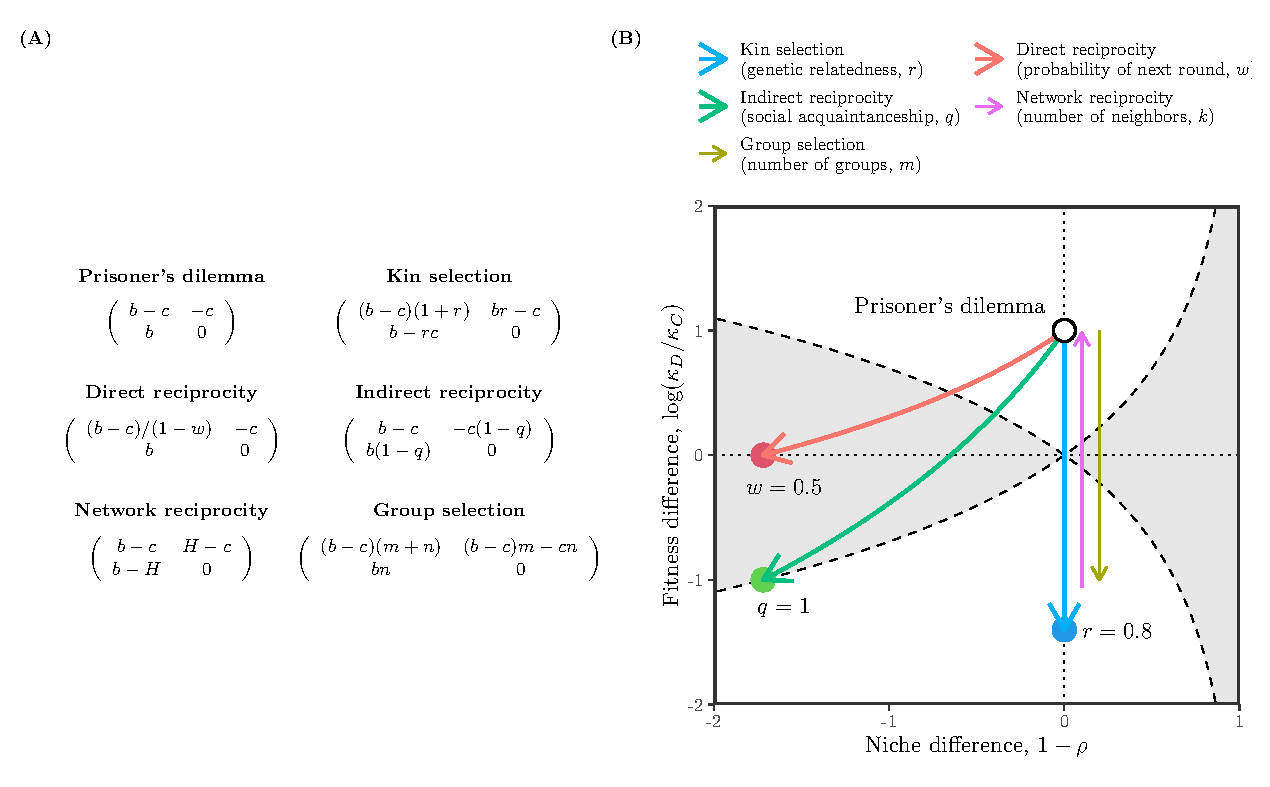
\includegraphics[width=\textwidth]{../diagram_cooperation/diagram_cooperation.pdf}
\caption{
\textbf{Qualitative comparisons of five mechanisms for the evolution of cooperation using SCT.}
(A) Payoff matrices for the baseline scenario (prisoner's dilemma) and five mechanisms for the evolution of cooperation  \citep{nowak2006five}.
Prisoner's dilemma is characterized by the benefit for the recipient $b$ and the cost for the donor $c$.
Network reciprocity is parameterized based on $H= [(b-c)k -2c]/[(k+1)(k-2)]$.
Parameters for all other mechanisms are described in panel B.
(B) Changes in niche and fitness differences driven by each mechanism.
Each arrow represents the direction of change as we increase the corresponding parameter, indicated in figure legends.
Note that kin selection, network reciprocity, and group selection all result in changes in fitness difference without causing any changes in niche difference.
Therefore, we indicate the direction of change for network reciprocity and group selection separately to avoid overlapping arrows.
For simplicity, we focus on the effect of number of groups $m$ for group selection; increasing the number of maximum group size $n$ has the opposite effect (Supplementary Text S4).
Across all models, we assume $b=3$ and $c=1$.
Because SCT decompositions depend on positive payoff scaling, exact values of niche and fitness difference (e.g., arrow lengths, slopes, and distances from regime boundaries) should not be compared across mechanisms.
}
\end{figure}

First, the prisoner's dilemma provides a baseline scenario, where defection is evolutionarily stable (Figure 3A).
From the perspective of SCT, there is complete niche overlap, and therefore defection competitively excludes cooperation (Figure 3B).
Building on this, SCT shows that five mechanisms promote evolutionary stability of cooperation via different dynamical routes  (Figure 3B).
For example, kin selection allows the fitness of cooperation to increase as genetic relatedness $r$ increases (Figure 3B).
However, it does not affect the niche difference between cooperation and defection.
Similarly, network reciprocity and group selection modulate the fitness of cooperation without causing any changes in strategic niches.
In contrast, direct and indirect reciprocity destabilize competition while increasing the fitness of cooperation, thereby pushing the competition outcome towards a priority effect regime.
Equivalently, these two mechanisms promote bistability of defection and cooperation.

SCT further illustrates another difference between direct and indirect reciprocity.
Direct reciprocity remains within the priority-effect regime as $w$ reaches 1, whereas indirect reciprocity reaches the boundary between the priority-effect and competitive-exclusion regimes at $q=1$ (Supplementary Text S4).

We note that none of these mechanisms allow coexistence of cooperation and defection.
In many biological systems, such coexistence is often observed \citep{gore2009snowdrift,cordero2012public,kocher2018genetic,pollak2021public,lin2024interspecific}.
Therefore, we move on to the next example, where environmental stochasticity can promote coexistence of cooperators and defectors.

\section*{Can stochasticity prevent coexistence?}

So far, we have focused on simple deterministic games. 
However, many ecological and evolutionary processes are intrinsically stochastic.
Recently, \cite{wang2025evolution} showed that environmental fluctuations can promote coexistence in games that would otherwise lead to competitive exclusion in a deterministic environment. 
From the perspective of SCT, this suggests that stochasticity can stabilize competition by promoting the recovery of strategies when rare.
Interestingly, \cite{wang2025evolution} also showed that stochasticity can generate bistable coexistence and multiple internal equilibria.
Thus, although stochasticity can stabilize competition near the boundaries, it can also generate destabilizing frequency dependence in the interior. 
This immediately raises the question of whether stochasticity can generate sufficiently strong positive frequency dependence to destabilize competition, thus pushing the system out of the coexistence regime.
Here, we use SCT to separate these effects and clarify whether stochasticity stabilizes or destabilizes strategic competition (Supplementary Text S5).
Although we refer to the two strategies as cooperation and defection for consistency, this analysis is not restricted to the Prisoner’s Dilemma and can be applied to any $2\times 2$ games.

Following \cite{wang2025evolution}, we consider a $2\times 2$ game in the presence of environmental noise. 
The stochastic payoff matrix is given by
\begin{equation}
\begin{pmatrix}
R & S \\
T & P
\end{pmatrix} +
\frac{\zeta}{\sqrt{s}} \begin{pmatrix}
\sigma_R & \sigma_S \\
\sigma_T & \sigma_P
\end{pmatrix}, 
\end{equation}
where the first matrix represents deterministic payoffs,
$\zeta$ represents a noise term with zero mean and unit variance,
and the second matrix determines the intensity of environmental stochasticity.
Assuming weak selection $s\ll 1$, the evolution of two competing strategies in a large population can be described by the following equation:
\begin{equation}
\frac{dx}{dt} = s x (1-x) \left(\pi_C - \pi_D + \left(\frac{1}{2} - x \right) (\sigma_C - \sigma_D)^2 \right),
\end{equation}
where $\pi_C = Rx + S(1-x)$ and $\pi_D = T x + P(1-x)$ and $\sigma_C = \sigma_R x + \sigma_S (1-x)$ and $\sigma_D = \sigma_T x + \sigma_P (1-x)$.
After rescaling time as $\tau = st$, the invasion growth rates of each strategy when rare can be written as:
\begin{align}
r_C &= S - P + \frac{1}{2}(\sigma_S - \sigma_P)^2,\\
r_D &= T - R + \frac{1}{2}(\sigma_T - \sigma_R)^2. 
\end{align}
This shows that invasion growth rates under environmental stochasticity will be greater than or equal to their deterministic counterparts, meaning that environmental stochasticity at the boundaries is intrinsically stabilizing.

Applying SCT, niche overlap and fitness difference for this system can be written as:
\begin{align}
\rho &= \exp\left(\frac{R+P-S-T}{2} - \frac{(\sigma_R - \sigma_T)^2 + (\sigma_S - \sigma_P)^2}{4} \right)\\
\frac{\kappa_D}{\kappa_C} &= \exp\left(\frac{T+P-R-S}{2} + \frac{(\sigma_R - \sigma_T)^2 - (\sigma_S - \sigma_P)^2}{4} \right)
\end{align}
Writing $\hat{\rho}$ and $\hat{\kappa}_D/\hat{\kappa}_C$ to denote niche overlap and fitness difference in the absence of stochasticity and taking logs of both sides for convenience, we have:
\begin{align}
\Delta \log \rho = \log \rho -  \log  \hat{\rho}&=- \frac{(\sigma_R - \sigma_T)^2 + (\sigma_S - \sigma_P)^2}{4}\\
\Delta \log \frac{\kappa_D}{\kappa_C} = \log \frac{\kappa_D}{\kappa_C}-\log \frac{\hat{\kappa}_D}{\hat{\kappa}_C} &= \frac{(\sigma_R - \sigma_T)^2 - (\sigma_S - \sigma_P)^2}{4}.
\end{align}
Therefore, stochasticity reduces niche overlap and increases niche difference.
In contrast, stochasticity can either amplify or reduce fitness differences depending on which strategy’s invasion rate is more strongly affected by environmental fluctuations.
Notably, changes in fitness difference driven by environmental stochasticity will always be bounded by those in niche overlap:
\begin{align}
\Delta \log \rho \leq \Delta \log \frac{\kappa_D}{\kappa_C} \leq - \Delta \log \rho
\end{align}
This result implies that environmental stochasticity cannot generate sufficient fitness difference to push the system out of the coexistence regime.

\begin{figure}[!th]
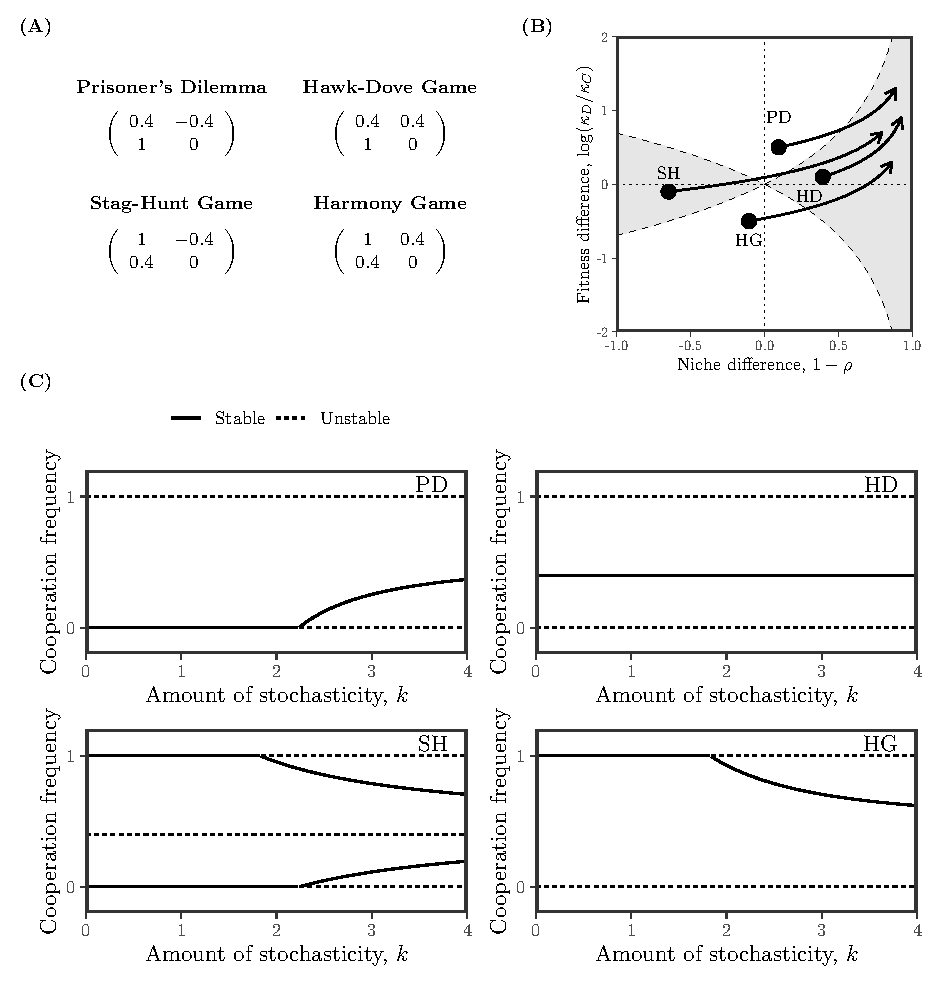
\includegraphics[width=\textwidth]{../diagram_stoch/diagram_stoch.pdf}
\caption{
\textbf{Effects of environmental stochasticity on strategic competition.}
(A) Assumed deterministic payoff structures across four scenarios.
Environmental stochasticity is assumed to be proportional to these payoffs, scaled by a term $k$.
(B) Arrows indicate the direction of changes in dynamical regime as the amount of stochasticity $k$ increases.
(C) Bifurcation diagrams under each scenario as a function of $k$. 
Solid and dashed lines represent stable and unstable equilibria, respectively.
}
\end{figure}

As an example, consider a scenario where the amount of stochasticity is assumed to be proportional to deterministic payoffs \citep{wang2025evolution}:
\begin{equation}
 \begin{pmatrix}
\sigma_R & \sigma_S \\
\sigma_T & \sigma_P
\end{pmatrix} =k \begin{pmatrix}
R & S \\
T & P
\end{pmatrix}.
\end{equation}
Following previous case studies, we consider four deterministic payoff structures (Figure 4A): Prisoner's Dilemma (PD), Hawk-Dove Game (HD), Stag-Hunt Game (SH) and Harmony Game (HG).
Across all these examples, stochasticity eventually pushes the system inside the mutual invasion regime (Figure 4B).
Notably, changes in dynamical regimes predicted by SCT accurately capture bifurcations occurring at the boundaries (Figure 4C): 
at sufficiently large $k$, both boundary equilibria are unstable in all four games.
Notably, for the SH game, the system begins from the priority effect regime and enters the competitive exclusion regime before eventually entering the mutual invasion regime (Figure 4B).
Consequently, $x=1$ (pure cooperation) becomes unstable first, and then $x=0$ (pure defection) also becomes unstable.

This example also illustrates an important limitation shared by MCT and SCT.
Since MCT and SCT solely rely on boundary conditions, they cannot predict the presence of multiple internal equilibria or their stability.
In the SH example, there is an unstable internal equilibrium across all ranges of $k$ we consider (Figure 4C).
When the system enters the competitive-exclusion regime, an additional stable internal equilibrium appears, allowing coexistence.
Furthermore, when mutual invasion is allowed, two stable coexistence equilibria are present.
Therefore, while MCT and SCT accurately capture the behavior at the boundary via invasibility, they do not fully characterize the interior dynamics or all conditions under which coexistence is possible.

\section*{Evolution of cooperation in multiplayer, nonlinear public goods games}

Previous case studies focused on evolutionary games based on pairwise interactions, but real-world behaviors, especially cooperation, often involve interactions among multiple players \citep{motro1991co,archetti2012game}.
In particular, cooperators can contribute to shared public goods, from which other individuals can benefit.
As our final study, we consider an N-player public-goods game to investigate the effects of multiplayer interaction on strategy competition.
In doing so, we also consider the effect of nonlinear public goods and ask when nonlinearity can stabilize or destabilize competition.

To model the evolution of cooperation under multiplayer interactions,
we begin by assuming that every individual receives the same amount of benefit $\beta(i)$ which increases monotonically with the number of cooperators $i$, and that cooperation incurs a constant cost $c > 0$.
Assuming that each individual interacts with $N-1$ other selected individuals, the average payoff for cooperators $\pi_C(x)$ and defectors $\pi_D(x)$ depends on the probability $f_j(x)$ of finding $j$ cooperators in the group, given $x$ proportion of cooperators in the population \citep{archetti2012game}:
\begin{align}
\pi_C(x) &= \sum_{j=0}^{N-1} f_j(x)\beta(j+1) -c\\
\pi_D(x) &= \sum_{j=0}^{N-1} f_j(x)\beta(j)
\end{align}
Assuming random, homogeneous mixing in a large population, the probability $f_j(x)$ follows a binomial distribution:
\begin{align}
\pi_C(x) &= \sum_{j=0}^{N-1} \binom{N-1}{j} x^j (1-x)^{N-1-j} \beta(j+1) -c\\
\pi_D(x) &= \sum_{j=0}^{N-1} \binom{N-1}{j} x^j (1-x)^{N-1-j}  \beta(j)
\end{align}
The resulting replicator equation corresponds to:
\begin{align}
\frac{dx}{dt} = x(1-x) G(x),
\end{align}
where $G(x) = \pi_C(x)-\pi_D(x)$ represents the payoff difference.

While this game consists of interactions between multiple individuals, from the perspective of SCT, there are still two strategies competing.
Thus, we can compute niche overlap $\rho$ and fitness difference $\kappa_D/\kappa_C$ using standard SCT, which in turn can be simplified in terms of payoff differences at the boundary:
\begin{align}
\rho &= \exp\left(\frac{\pi_C(1)+\pi_D(0)-\pi_C(0)-\pi_D(1)}{2}\right) = \exp\left(\frac{G(1)-G(0)}{2}\right)\\
\frac{\kappa_D}{\kappa_C} &= \exp\left(\frac{\pi_D(0)+\pi_D(1)-\pi_C(1)-\pi_C(0)}{2}\right) = \exp\left(-\frac{G(1)+G(0)}{2}\right).
\end{align}
Here, the payoff values at the boundary correspond to: 
\begin{align}
G(0) &= \beta(1) - \beta(0) -c\\
G(1) &= \beta(N) - \beta(N-1) - c
\end{align}
Finally, mutual invasion at the boundary requires:
\begin{align}
\rho < \frac{\kappa_D}{\kappa_C} < \frac{1}{\rho}.
\end{align}
This expression can be equivalently written as:
\begin{align}
G(1) < 0 < G(0) \iff \beta(N) - \beta(N-1) < c < \beta(1) - \beta(0).
\end{align}
This formulation shows that mutual invasion is possible only when the marginal benefit generated by the first cooperator exceeds that generated by the \(N\)th cooperator, with the cost of cooperation lying between these two marginal benefits.

We can now draw three conclusions from this observation.
First, when the benefit of public good $\beta(i)$ increases linearly with $i$ (thus $\beta(1) - \beta(0) = \beta(N) - \beta(N-1)$), then there is complete niche overlap because $G(1) = G(0)$.
In this case, cooperators competitively exclude defectors when the marginal benefit $\beta(1) - \beta(0)$ is greater than the cost $c$, and defectors competitively exclude cooperators when the marginal benefit is smaller than the cost.
Stable coexistence becomes impossible.
Second, when the benefit of public good $\beta(i)$ is a concave, increasing function of $i$ (i.e., $d\beta/di > 0$ and $d^2\beta/di^2 < 0$), we have $\beta(1)-\beta(0) >  \beta(N) - \beta(N-1)$ \citep{motro1991co}.
This means that nonlinearity can generate niche difference and allow coexistence when
\begin{equation}
\beta(N) - \beta(N-1) < c < \beta(1) - \beta(0)
\end{equation}
This generalizes the result of \cite{gore2009snowdrift}, showing that the effect of concave nonlinearity on coexistence is robust to multiplayer extension (see Supplementary Text S6 and Figure S1 for detailed analyses).
Third, when the benefit of public good $\beta(i)$ is a convex, increasing function of $i$ (i.e., $d\beta/di > 0$ and $d^2\beta/di^2 > 0$), we have $\beta(1)-\beta(0) < \beta(N) - \beta(N-1)$ \citep{motro1991co}.
In this case, nonlinearity can allow bistability of two boundary monomorphic equilibria and generate priority effect when
\begin{equation}
\beta(1) - \beta(0) < c < \beta(N) - \beta(N-1).
\end{equation}
Therefore, SCT shows that nonlinearity can either stabilize or destabilize strategic coexistence depending on the shape of nonlinearity.
Accordingly, $G(x)$ decreases monotonically for concave benefits and increases monotonically for convex benefits, so these cases can have at most one internal equilibrium.

We note that this multiplayer game can also permit multiple internal equilibria.
For example, \cite{archetti2012game} considers a scenario where $\beta(t)$ follows a sigmoid function, illustrating that coexistence between cooperators and defectors is possible even when defectors have higher payoffs at both boundaries.
In such cases, SCT will be able to capture invasibility at the boundary but will not be able to predict internal dynamics, as we show in the previous case study.

\section*{Discussion}

Standard evolutionary game theory and replicator equations provide powerful tools for predicting the outcome of strategy competition, including strategic dominance, coexistence, and bistability \citep{motro1991co,doebeli2004evolutionary,hauert2004spatial,doebeli2005models,gore2009snowdrift,souza2009evolution,archetti2011coexistence,steidinger2014coexistence,tarnita2025reconciling}.
However, these outcomes are typically understood by analyzing payoff differences within individual games, which makes it difficult to compare coexistence mechanisms across models.
Building on Chesson's Modern Coexistence Theory from community ecology \citep{chesson2000mechanisms}, we developed a strategic coexistence theory (SCT) that allows us to decompose strategy competition at the invasion boundaries in terms of stabilizing niche differences and fitness differences.

To demonstrate the utility of SCT, we considered four case studies.
First, the analysis of classic two-strategy games showed that SCT recovers the original classification for these classic games, highlighting the similarities between evolutionary games and community ecology \citep{hauert2002effects,szabo2007evolutionary,cooney2020analysis,tarnita2025reconciling}.
Second, we compared different mechanisms for the evolution of cooperation, which showed that each mechanism promotes cooperation via different dynamical routes \citep{nowak2006five}.
Kin selection, network reciprocity, and group selection primarily affect the fitness difference between cooperation and defection, whereas direct and indirect reciprocity can destabilize competition and generate priority effects.
Third, we considered the effect of environmental stochasticity on strategy competition, showing that stochasticity cannot destabilize competition.
Finally, a case study of multiplayer, public-goods games showed that nonlinear public benefit can either stabilize or destabilize competition.
The final two applications also revealed an important limitation of analyses based on invasion growth rates at monomorphic boundary conditions: they are unable to predict the number or stability of interior equilibria.
We note that SCT is not intended to produce dynamical predictions that differ from standard analyses in EGT.
Instead, SCT provides a common visualization and expository framework for comparing how different mechanisms alter boundary invasibility through changes in strategic niche and fitness differences.

There are several limitations to SCT.
First, similar to MCT in community ecology, SCT only allows for comparisons of pairwise strategies and therefore cannot determine the outcomes of games with more than two strategies \citep{chesson2000mechanisms}.
While SCT can be still applied to multi-player interactions, conclusions based on 2-player games may not be robust to multi-player extensions, which can introduce nonlinearity.
Thus, our analysis of cooperation mechanisms should be interpreted as specific to the pairwise formulations considered here and as an illustration of SCT, rather than as general conclusions about multiplayer versions of these mechanisms.

Second, the exact values of strategic niche and fitness differences are sensitive to payoff scaling.
SCT therefore supports quantitative comparisons only when models share a justified payoff normalization. 
Without such normalization, comparisons are restricted to qualitative changes in dynamical regimes, directions, and boundary crossings. 

Third, we focused on classic replicator equations, but \cite{tarnita2025reconciling} recently pointed out that these classic formulations implicitly ignore differences in intrinsic growth rates.
In such cases, replicator equations may fail to predict the outcome of competition \citep{tarnita2025reconciling}, and a full Lotka-Volterra model is needed to describe the abundances, rather than frequencies, of strategies.
Thus, SCT inherits the same assumptions as the classic replicator framework: it is most appropriate when strategy competition can be described in terms of relative frequencies alone \citep{tarnita2025reconciling}.
When strategies differ intrinsically in growth, MCT may be required instead to tease apart mechanisms of strategy coexistence.

Finally, we have focused on simple examples to illustrate the utility of SCT, but many games involve additional complexities, including population structure \citep{nowak2010evolutionary} and explicit ecological feedback \citep{weitz2016oscillating,tarnita2025reconciling}.
Extending SCT to these settings will be necessary to determine how broadly stabilizing and equalizing mechanisms can be compared across evolutionary games.

While SCT was inspired by MCT, there are important differences between the two frameworks.
In particular, MCT describes changes in species abundance, whereas SCT describes changes in strategy frequency.
For example, even when growth rates of the abundances of both competitors are negative, the growth rate of the frequency of a superior competitor will still be positive;
this implies that the invasibility in frequency and abundance space are fundamentally different.
Moreover, MCT relies on a simple, Lotka-Volterra model, which permits at most one internal equilibrium, which allows us to predict coexistence from mutual invasion.
However, SCT relies on replicator dynamics, which can permit multiple internal equilibria, meaning that criterion for mutual invasion and coexistence can differ.
Therefore, SCT should be interpreted as a decomposition framework that is inspired by MCT, rather than a direct extension.

In conclusion, SCT provides a bridge between evolutionary game theory and community ecology, allowing strategy competition to be understood from the perspective of coexistence theory. 
Therefore, rather than replacing existing EGT or replicator-dynamics frameworks, SCT provides a complementary tool for teasing apart the coexistence mechanisms underlying evolutionary games.
More broadly, our study builds on recent efforts to extend MCT beyond species competition \citep{park2024predicting,park2026unifying}, providing a foundation for building unifying coexistence theory for competing entities, including species, pathogen strains, and behavioral strategies.

\section*{Acknowledgement}

We thank Jonathan Levine for the helpful discussion.
S.W.P. was supported by the New Faculty Startup Fund from Seoul National University,
the National Research Foundation of Korea (NRF) grant funded by the Korea government (MSIT) (RS-2026-25474574),
and the Global-LAMP Program of the National Research Foundation of Korea (NRF) grant funded by the Ministry of Education (No. RS-2023-00301976).

\section*{Competing interests}

The authors declare no competing interest.

\section*{Data availability}

All data and code are stored in a publicly available GitHub repository (\url{https://github.com/parklab-snu/coexistence-strategy}).

\pagebreak

\renewcommand\theequation{S\arabic{equation}}    
\setcounter{equation}{0}

\section*{Supplementary Text}

\subsection*{S1 Derivation of the strategic coexistence theory}

To derive strategic coexistence theory (SCT), we begin with replicator equations:
\begin{align}
\frac{dx_i}{dt} &= x_i (\pi_i(\mathbf{x}) - \bar{\pi}(\mathbf{x})),
\end{align}
where $x_i$ represents the frequency of strategy $i$, $\pi_i$ represents the payoff of strategy $i$, and $\bar{\pi}$ represents the average payoff.
Then, the mutual invasion condition for two competing strategies $i$ and $j$ can be written as
\begin{align}
\pi_j(\mathbf{e}_j) & <\pi_i(\mathbf{e}_j),\\
\pi_i(\mathbf{e}_i) &< \pi_j(\mathbf{e}_i).
\end{align}
These inequalities will be preserved when we exponentiate the payoffs, $W_i(\mathbf{x}) = \exp(\pi_i(\mathbf{x}))$:
\begin{align}
W_j(\mathbf{e}_j) &< W_i(\mathbf{e}_j),\\
W_i(\mathbf{e}_i) &< W_j(\mathbf{e}_i).
\end{align}
Rearranging, we obtain the following inequality:
\begin{align}
\frac{W_i(\mathbf{e}_i)}{W_j(\mathbf{e}_i)} < 1 < 
\frac{W_i(\mathbf{e}_j)}{W_j(\mathbf{e}_j)}.
\end{align}
By multiplying $\sqrt{\frac{W_j(\mathbf{e}_i)W_j(\mathbf{e}_j) }{W_i(\mathbf{e}_i) W_i(\mathbf{e}_j)}}$ on both sides, we obtain:
\begin{equation}
\sqrt{\frac{W_i(\mathbf{e}_i) W_j(\mathbf{e}_j)}{  W_j(\mathbf{e}_i)W_i(\mathbf{e}_j)}} < 
\sqrt{\frac{W_j(\mathbf{e}_i)W_j(\mathbf{e}_j) }{W_i(\mathbf{e}_i) W_i(\mathbf{e}_j)}}
< 
\sqrt{\frac{W_j(\mathbf{e}_i)W_i(\mathbf{e}_j)}{W_i(\mathbf{e}_i) W_j(\mathbf{e}_j) } }
\end{equation}
Thus, by defining niche overlap $\rho$ and fitness difference $\kappa_j/\kappa_i$ as follows,
\begin{align}
\rho &= \sqrt{\frac{W_i(\mathbf{e}_i) W_j(\mathbf{e}_j)}{W_j(\mathbf{e}_i) W_i(\mathbf{e}_j) }},\\
\frac{\kappa_j}{\kappa_i} &= \sqrt{\frac{W_j(\mathbf{e}_i)W_j(\mathbf{e}_j) }{W_i(\mathbf{e}_i) W_i(\mathbf{e}_j)}},
\end{align}
we obtain the following inequality that defines conditions for mutual invasion:
\begin{equation}
\rho < \frac{\kappa_j}{\kappa_i} < \frac{1}{\rho}.
\end{equation}

Note that mutual invasion condition can be also written in terms of invasion growth rates at monomorphic equilibrium $r_{i|j}$ and $r_{j|i}$:
\begin{align}
0 &< r_{i|j},\\
0 &< r_{j|i}.
\end{align}
Analogous to the previous derivation, the mutual condition can be then rewritten as:
\begin{align}
-\frac{r_{j|i}+r_{j|i}}{2} < \frac{r_{j|i}-r_{j|i}}{2} < \frac{r_{i|j} + r_{j|i}}{2}.
\end{align}
Exponentiating all sides preserves the inequality and keep them positive:
\begin{align}
\exp\left(-\frac{r_{j|i}+r_{j|i}}{2}\right) < \exp\left(\frac{r_{j|i}-r_{j|i}}{2}\right) < \exp\left(\frac{r_{i|j} + r_{j|i}}{2}\right).
\end{align}
Thus, by defining niche overlap $\rho$ and fitness difference $\kappa_j/\kappa_i$ as follows,
\begin{align}
\rho &= \exp\left(-\frac{r_{j|i}+r_{j|i}}{2}\right),\\
\frac{\kappa_j}{\kappa_i} &= \exp\left(\frac{r_{j|i}-r_{j|i}}{2}\right),
\end{align}
we obtain the following inequality that defines conditions for mutual invasion:
\begin{equation}
\rho < \frac{\kappa_j}{\kappa_i} < \frac{1}{\rho}.
\end{equation}

\subsection*{S2 Niche and fitness difference payoff scaling}

Consider a classic replicator equation:
\begin{align}
\frac{dx_i}{dt} &= x_i (\pi_i(\mathbf{x}) - \bar{\pi}(\mathbf{x})),
\end{align}
where $x_i$ represents the frequency of strategy $i$, $\pi_i$ represents the payoff of strategy $i$, and $\bar{\pi}$ represents the average payoff.
In this case, multiplying the payoffs by a constant $s > 0$ only changes time and does not affect the overall dynamics:
\begin{align}
\frac{dx_i}{dt} &= x_i (\pi'_i(\mathbf{x}) - \bar{\pi'}(\mathbf{x}))\\
&= s x_i (\pi_i(\mathbf{x}) - \bar{\pi}(\mathbf{x})),
\end{align}
where $\pi'_i(\mathbf{x}) = s \pi(\mathbf{x})$ is the scaled payoff.
Then, the multiplicative payoff corresponds to $W_i'(\mathbf{x}) = \exp(s\pi_i) = W_i(\mathbf{x})^s$.

If we try to calculate niche overlap and fitness difference based on the scaled payoffs, we get:
\begin{align}
\rho' &= \sqrt{\frac{W_i'(\mathbf{e}_i) W_j'(\mathbf{e}_j)}{W_j'(\mathbf{e}_i) W_i'(\mathbf{e}_j) }},\\
&= \left(\sqrt{\frac{W_i(\mathbf{e}_i) W_j(\mathbf{e}_j)}{W_j(\mathbf{e}_i) W_i(\mathbf{e}_j)}}\right)^s,\\
&= \rho^s\\
\frac{\kappa_j'}{\kappa_i'} &= \sqrt{\frac{W_j'(\mathbf{e}_i)W_j'(\mathbf{e}_j) }{W_i'(\mathbf{e}_i) W_i'(\mathbf{e}_j)}},\\
&=  \left(\sqrt{\frac{W_j(\mathbf{e}_i)W_j(\mathbf{e}_j) }{W_i(\mathbf{e}_i) W_i(\mathbf{e}_j)}}\right)^s,\\
&= \left(\frac{\kappa_j}{\kappa_i}\right)^s
\end{align}
This implies that the exact values of niche and fitness difference are sensitive to payoff scaling and are not intrinsic properties of a replicator system.

Nonetheless, the inequality for mutual invasion condition still holds under payoff scaling:
\begin{equation}
\rho < \frac{\kappa_j}{\kappa_i} < \frac{1}{\rho} \iff \rho^s < \left(\frac{\kappa_j}{\kappa_i}\right)^s < \frac{1}{\rho^s}.
\end{equation}
Furthermore, boundary conditions for complete niche overlap ($\rho=\rho'=1$) and complete niche difference ($\rho=\rho'=0$) are preserved.
Moreover, the direction of changes in fitness and niche difference is also preserved under payoff scaling.
Specifically, for parameter $\theta$, we have:
\begin{align}
\frac{d\rho'}{d\theta} &= s \rho^{s-1} \frac{d\rho}{d\theta}\\ 
\frac{d}{d\theta}\left(\frac{\kappa_j'}{\kappa_i'}\right) &= s \left(\frac{\kappa_j}{\kappa_i}\right)^{s-1} \frac{d}{d\theta}\left(\frac{\kappa_j}{\kappa_i}\right).
\end{align}
Since $\rho$ and $\kappa_j/\kappa_i$ are always positive, directional sensitivities of $\rho$ and $\kappa_j/\kappa_i$ to parameter $\theta$ are preserved.
Similarly, directional sensitivities of $1-\rho$ to $\theta$ are preserved:
\begin{align}
\frac{d(1-\rho')}{d\theta} &= s \rho^{s-1} \frac{d(1-\rho)}{d\theta}
\end{align}
Therefore, we focus on comparisons of qualitative outcomes from SCT and refrain from making any comparisons of magnitude of niche and fitness difference values.

\subsection*{S3 Applications to classic two-strategy games}

Consider a two-strategy game described by the following payoff matrix:
\begin{equation}
\begin{pmatrix}
R & S \\
T & P
\end{pmatrix}.
\end{equation}
There are four classic games that we can define from this simple payoff matrix:
prisoner’s dilemma ($T>R > P>S$), hawk--dove game ($T>R$, $S>P$), stag--hunt game ($R>T$, $P>S$), and harmony game ($R>T$, $S>P$). 
Here, we show that each game corresponds to a distinct region in the niche-fitness difference space under SCT.

To do so, we first begin by deriving expressions for niche overlap $\rho$ and fitness difference $\kappa_j/\kappa_i$.
Writing $x_1$ to denote the frequency of strategy 1, the expected payoff for each strategy corresponds to:
\begin{align}
\pi_1(\mathbf{x}) &= R x_1 + S(1-x_1),\\
\pi_2(\mathbf{x}) &= T x_1 + P(1-x_1).
\end{align}
Then, multiplicative payoffs for each strategy when rare can be written as:
\begin{align}
W_1(1) &= \exp(R)\\
W_1(0) &= \exp(S)\\
W_2(1) &= \exp(T)\\
W_2(0) &= \exp(P)
\end{align}
Therefore, we have:
\begin{align}
\rho &= \exp\left(\frac{R + P - S - T}{2}\right),\\
\frac{\kappa_2}{\kappa_1} &= \exp\left(\frac{T+P-R-S}{2}\right).
\end{align}
As before, the mutual-invasion condition can be expressed as:
\begin{equation}
\rho < \frac{\kappa_j}{\kappa_i} < \frac{1}{\rho}.
\end{equation}

Then, simple algebra reveals that each condition in mutual invasion inequality can be equivalently described by the payoff inequality:
\begin{align}
\rho < \frac{\kappa_2}{\kappa_1} &\iff R < T\\
\rho > \frac{\kappa_2}{\kappa_1} &\iff R > T\\
\frac{\kappa_2}{\kappa_1} < \frac{1}{\rho} &\iff P < S\\
\frac{\kappa_2}{\kappa_1} > \frac{1}{\rho} &\iff P > S
\end{align}
These inequalities then allow us to classify outcomes of two-strategy games from the perspective of SCT.
Note that the inequality between $R$ and $P$ does not affect the outcome.

\subsection*{S4 Applications to mechanisms for the evolution of cooperation}

We consider five mechanisms for the evolution of cooperation, all of which can be represented as a simple $2\times 2$ payoff matrix \citep{nowak2006five}.
Here, we go through each mechanism and derive measures for niche and fitness differences.

\textbf{Prisoner's dilemma.}
Here, we consider a special case of Prisoner's dilemma which can be described by the following payoff matrix:
\begin{equation}
\begin{pmatrix}
b-c & -c \\
b & 0
\end{pmatrix},
\end{equation}
where $b$ represents the benefit for the recipient and $c$ represents cost for the donor.
In this case, the niche and fitness differences correspond to:
\begin{align}
1-\rho &= 0\\
\frac{\kappa_2}{\kappa_1} &= \exp\left(c\right).
\end{align}
Therefore, as long as the cost is greater than zero, prisoner's dilemma always results in the competitive exclusion of cooperation.

\textbf{Kin selection.}
Kin selection can be described by the following payoff matrix:
\begin{equation}
\begin{pmatrix}
(b-c)(1+r) & br-c \\
b-rc & 0
\end{pmatrix},
\end{equation}
where $r$ represents the genetic relatedness. 
In this case, the niche and fitness differences correspond to:
\begin{align}
1-\rho &= 0\\
\frac{\kappa_2}{\kappa_1} &= \exp\left(c-br\right).
\end{align}
Therefore, defection will exclude cooperation when $c > br$. Equivalently, cooperation will be favored when $r > c/b$, which recovers the classic result.

\textbf{Direct reciprocity.}
Direct reciprocity can be described by the following payoff matrix:
\begin{equation}
\begin{pmatrix}
(b-c)/(1-w) & -c \\
b & 0
\end{pmatrix},
\end{equation}
where $w$ represents the probability of next round. 
In this case, the niche and fitness differences correspond to:
\begin{align}
1-\rho &= 1- \exp\left(\frac{(b-c)/(1-w) + c - b}{2}\right) \\
\frac{\kappa_2}{\kappa_1} &= \exp\left(\frac{b+c-(b-c)/(1-w)}{2}\right).
\end{align}
Therefore, defection will exclude cooperation when 
\begin{align}
\rho &< \frac{\kappa_2}{\kappa_1}\\
\iff \exp\left(\frac{(b-c)/(1-w) + c - b}{2}\right) &< \exp\left(\frac{b+c-(b-c)/(1-w)}{2}\right)\\
\iff bw &< c
\end{align}

However, note that the following inequality holds whenever $c > 0$:
\begin{align}
\frac{1}{\rho} &< \frac{\kappa_2}{\kappa_1}.
\end{align}
Therefore, when $w > c/b$, we will have
\begin{align}
\frac{1}{\rho} < \frac{\kappa_2}{\kappa_1} < \rho,
\end{align}
which implies priority effect (equivalently, bistability).
Even as $w \to 1^-$, this inequality holds and therefore, cooperation cannot competitively exclude defection.

\textbf{Indirect reciprocity.}
Indirect reciprocity can be described by the following payoff matrix:
\begin{equation}
\begin{pmatrix}
b-c & -c(1-q) \\
b(1-q) & 0
\end{pmatrix},
\end{equation}
where $q$ represents social acquaintanceship.
In this case, the niche and fitness differences correspond to:
\begin{align}
1-\rho &= 1- \exp\left(\frac{(b-c)q}{2}\right),\\
\frac{\kappa_2}{\kappa_1} &= \exp\left(\frac{2c-(b+c)q}{2}\right).
\end{align}
In this case, the condition for the dominance of defection (and therefore competitive exclusion of cooperation) can be written as:
\begin{align}
\rho &< \frac{\kappa_2}{\kappa_1}\\
\iff bq  &< c
\end{align}
Moreover, the following inequality always holds as long as $c > 0$.
\begin{align}
\frac{1}{\rho} &< \frac{\kappa_2}{\kappa_1},
\end{align}
which implies that coexistence between cooperation and defection is not possible.
Therefore, when $q < c/b$, then defection will competitively exclude cooperation. 
Otherwise, the system will enter the priority-effect regime.

Interestingly, when $q \to 1$, we have 
\begin{align}
\rho &= \exp\left(\frac{b-c}{2}\right)\\
\frac{\kappa_2}{\kappa_1} &= \exp\left(\frac{c-b}{2}\right)\\
\frac{1}{\rho} &= \exp\left(\frac{c-b}{2}\right)\\
\end{align}
In other words, the following inequality will hold:
\begin{align}
\frac{1}{\rho} = \frac{\kappa_2}{\kappa_1} < \rho 
\end{align}

\textbf{Network reciprocity.} Network reciprocity can be described by the following payoff matrix:
\begin{equation}
\begin{pmatrix}
b-c & H-c \\
b-H & 0
\end{pmatrix},
\end{equation}
where $H= [(b-c)k -2c]/[(k+1)(k-2)]$ and $k$ represents the number of neighbors. 
In this case, the niche and fitness differences correspond to:
\begin{align}
1-\rho &= 0,\\
\frac{\kappa_2}{\kappa_1} &= \exp\left(-H+c\right),
\end{align}
which implies that there is complete niche overlap and that fitness difference decreases with $H$.
Since $H$ is a monotonically decreasing function of $k$ when $k > 2$ and $b/c \geq 2$, fitness difference will increase with $k$.
In particular, cooperation will competitively exclude defection when $H>c$, meaning that:
\begin{equation}
b/c > k.
\end{equation}

\textbf{Group selection.} Group selection can be described by the following payoff matrix:
\begin{equation}
\begin{pmatrix}
(b-c)(m+n) & (b-c)m - cn \\
bn & 0
\end{pmatrix},
\end{equation}
where $m$ represents the number of groups and $n$ represents the group size.
In this case, the niche and fitness differences correspond to:
\begin{align}
1-\rho &= 0,\\
\frac{\kappa_2}{\kappa_1} &= \exp\left((c-b)m+cn \right),
\end{align}
which implies that there is complete niche overlap.
The fitness difference will increase with $n$ but decrease with $m$, provided that $b > c$.
In particular, cooperation will competitively exclude defection under the following condition:
\begin{equation}
1+ \frac{n}{m} < \frac{b}{c}.
\end{equation}

\section*{S5 Applications to evolutionary games with environmental stochasticity}


Consider a competition of two strategies under stochastic payoffs:
\begin{equation}
\begin{pmatrix}
R & S \\
T & P
\end{pmatrix} +
\frac{\zeta}{\sqrt{s}} \begin{pmatrix}
\sigma_R & \sigma_S \\
\sigma_T & \sigma_P
\end{pmatrix}, 
\end{equation}
Assuming weak selection $s\ll 1$, the evolution of two competing strategies in a large population can be described by the following equation:
\begin{equation}
\frac{dx}{dt} = s x (1-x) \left(\pi_C - \pi_D + \left(\frac{1}{2} - x \right) (\sigma_C - \sigma_D)^2 \right),
\end{equation}
To simplify, we write
\begin{equation}
\frac{dx}{dt} = s x (1-x) G(x),
\end{equation}
where
\begin{equation}
G(x) = \left(\pi_C - \pi_D + \left(\frac{1}{2} - x \right) (\sigma_C - \sigma_D)^2 \right).
\end{equation}
Thus, the sign of $G(x)$ at boundary conditions determines whether a strategy can invade when the competing strategy is at equilibrium.

Since $G(x)$ does not uniquely separate into two payoff measures, we define niche and fitness difference based on the invasion growth rates $r_{C|D} = G(0)$ and $r_{D|C} = -G(1)$:
\begin{align}
1 -\rho &= - \exp\left(\frac{G(1)-G(0)}{2}\right)\\
\frac{\kappa_D}{\kappa_C} &= \exp\left(-\frac{G(1)+G(0)}{2}\right)
\end{align}
Then, by substituting expressions for $G(0)$ and $G(1)$, we obtain the following expressions for niche and fitness difference:
\begin{align}
1- \rho &= 1-\exp\left(\frac{R+P-S-T}{2} - \frac{(\sigma_R - \sigma_T)^2 + (\sigma_S - \sigma_P)^2}{4} \right)\\
\frac{\kappa_D}{\kappa_C} &= \exp\left(\frac{T+P-R-S}{2} + \frac{(\sigma_R - \sigma_T)^2 - (\sigma_S - \sigma_P)^2}{4} \right)
\end{align}

Now, to study the interior behavior of the system, we assume that the amount of stochasticity is proportional to deterministic payoffs \citep{wang2025evolution}:
\begin{equation}
 \begin{pmatrix}
\sigma_R & \sigma_S \\
\sigma_T & \sigma_P
\end{pmatrix} =k \begin{pmatrix}
R & S \\
T & P
\end{pmatrix}.
\end{equation}
Then, the expression for $G(x)$ can be written as:
\begin{align}
G(x) &= \left( (R-T)x + (S-P)(1-x) \right) \times\\
&\quad{}\left(1+ k^2 \left(\frac{1}{2} - x \right) ((R-T)x + (S-P)(1-x))\right)\\
&= \left( (R+P-T-S)x + (S-P) \right) \times\\
&\quad{}\left(1+ k^2 \left(\frac{1}{2} - x \right) ((R+P-T-S)x + (S-P))\right)\\
&= k^2 (R+P-T-S)^2 \left(x-x^\ast \right) \left(K + \left(\frac{1}{2} - x \right) (x - x^\ast)\right),
\end{align}
where $x^\ast = (P-S)/(R+P-T-S)$ and $K = 1/(k^2(R+P-T-S))$ for $k > 0$ and $R + P -T - S \neq 0$.
Therefore, this system has an internal equilibrium $x=x^\ast$ when $0 < (P-S)/(R+P-T-S) < 1$.

The system can also have up to two additional equilibria when $K + \left(\frac{1}{2} - x \right) (x - x^\ast) = 0$ has positive, real roots and when these roots fall between 0 and 1.
In particular, the quadratic equation can be written as:
\begin{equation}
x^2 -\left(\frac{1}{2} + x^\ast \right) x + \frac{x^\ast}{2} - K = 0.
\end{equation}
Thus, the two solutions of the quadratic equation correspond to:
\begin{equation}
x = \frac{x^\ast + \frac{1}{2} \pm \sqrt{\left(\frac{1}{2} - x^\ast \right)^2 + 4K}}{2}.
\end{equation}
These solutions are real when:
\begin{equation}
\left(\frac{1}{2} - x^\ast \right)^2 + 4K > 0.
\end{equation}
When these solutions fall between 0 and 1, they correspond to additional internal equilibria.

\section*{S6 Microbial cooperation and public goods}

Here, we consider a simple, phenomenological model of competition between cooperating and cheating yeast in a cooperative sucrose-metabolism system, where invertase production by cooperators allows cheaters to utilize glucose, a public good released through sucrose hydrolysis \citep{carlson1982two,dickinson1998metabolism,gore2009snowdrift}.
We note that this is a phenomenological approximation of a public-goods game as it does not explicitly consider interactions between multiple players \citep{archetti2011coexistence}.
Nonetheless, this example provides a simple illustration of how a concave benefit function can promote coexistence.

Invertase production by cooperators incurs a cost $c$ and generates a total benefit of 1 that is captured privately with efficiency $\epsilon$. 
Assuming a linear relationship between glucose availability and microbial growth, the payoffs for cooperators $\pi_C$ and cheaters (defectors) $\pi_D$ can then be written as
\begin{align}
\pi_C(f) &= \epsilon + f (1-\epsilon) - c,\\
\pi_D(f) &= f (1-\epsilon),
\end{align}
where the use of glucose depends on the fraction of cooperators $f$. 
The dynamics of cooperators and defectors are described by the following replicator equation:
\begin{align}
\frac{df}{dt} &= f(1-f)\left[\pi_C(f)-\pi_D(f)\right]\\
&= f(1-f)(\epsilon - c)
\end{align}
For this linear growth model, the payoff difference is fixed to $\epsilon-c$ independent of $f$ (Figure S1A).
Therefore, cooperation is favored when efficiency is greater than the cost of cooperation, $\epsilon > c$, whereas defection is favored when the cost is greater than efficiency, $c > \epsilon$ \citep{gore2009snowdrift}.

Our framework allows us to reinterpret this result from the perspective of coexistence theory. 
In particular, the two strategies have no niche difference, corresponding to complete niche overlap, $\rho = 1$. 
In contrast, the fitness difference is determined by the balance between private efficiency and the cost of cooperation:
\begin{equation}
\frac{\kappa_D}{\kappa_C} = \exp(c - \epsilon).
\end{equation}
Therefore, this model always predicts competitive exclusion, except in the neutral case $c=\epsilon$. 
The outcome is determined entirely by the fitness difference between cooperators and defectors, rather than by stabilizing niche differences.

In real biological systems, the effect of glucose on microbial growth follows a nonlinear relationship:
\begin{align}
\pi_C(f) &= \left[\epsilon + f (1-\epsilon)\right]^\alpha - c,\\
\pi_D(f) &= [f (1-\epsilon)]^\alpha,
\end{align}
where $\alpha=0.15$ reflects the experimental relationship between glucose and microbial growth \citep{gore2009snowdrift}. 
Then, the dynamics of cooperators and defectors are described by the following replicator equation:
\begin{align}
\frac{df}{dt} &= f(1-f)\left[\left\{\epsilon + f (1-\epsilon)\right\}^\alpha - c - \{f (1-\epsilon)\}^\alpha \right].
\end{align}
Under this nonlinear assumption, the payoff difference decreases with the cooperator fraction $f$, which can promote the coexistence of cooperators and defectors (Figure S1A): cooperators have a competitive advantage when rare, whereas defectors have a competitive advantage when cooperators are abundant.
Because the payoff difference decreases monotonically with $f$, this model can have at most one internal equilibrium.
Thus, while it provides a simple illustration of how concavity can promote coexistence, it cannot capture the multiple internal equilibria that can arise under more general nonlinear benefit functions, such as sigmoid functions.

From a coexistence-theoretic perspective, this means that nonlinear growth can generate sufficient stabilizing niche difference to overcome the fitness difference. 
In particular, the niche and fitness differences for this model correspond to:
\begin{align}
1- \rho &= 1- \exp\left(\frac{1 - \epsilon^\alpha - (1-\epsilon)^\alpha }{2}\right),\\
\frac{\kappa_D}{\kappa_C} &= \exp\left(c + \frac{(1-\epsilon)^\alpha - 1 - \epsilon^{\alpha} }{2} \right).
\end{align}
These expressions clarify the separate roles of cost, efficiency, and nonlinearity.
For example, the cost of cooperation does not affect niche difference and only affects fitness difference.  
Instead, niche difference is generated by the concave relationship between glucose availability and microbial growth, which increases from 0 to $1-\exp(-1/2)$ as $\alpha$ goes from 1 to 0  (Figure S1B,C).
In contrast, as $\alpha \to 0^+$, the fitness difference approaches 
\begin{equation}
\log(\kappa_D/\kappa_C) \to c-\frac{1}{2},
\end{equation}
which no longer depends on the private capture efficiency $\epsilon$ (Figure S1C). 
Thus, strong concavity not only generates stabilizing niche differences, but also acts as an equalizing mechanism (Figure S1C).
Such stabilizing mechanisms are key ingredients for coexistence of competing strategies.

\pagebreak

\section*{Supplementary Figure}

\renewcommand\thefigure{S\arabic{figure}}    
\setcounter{figure}{0}

\begin{figure}[!th]
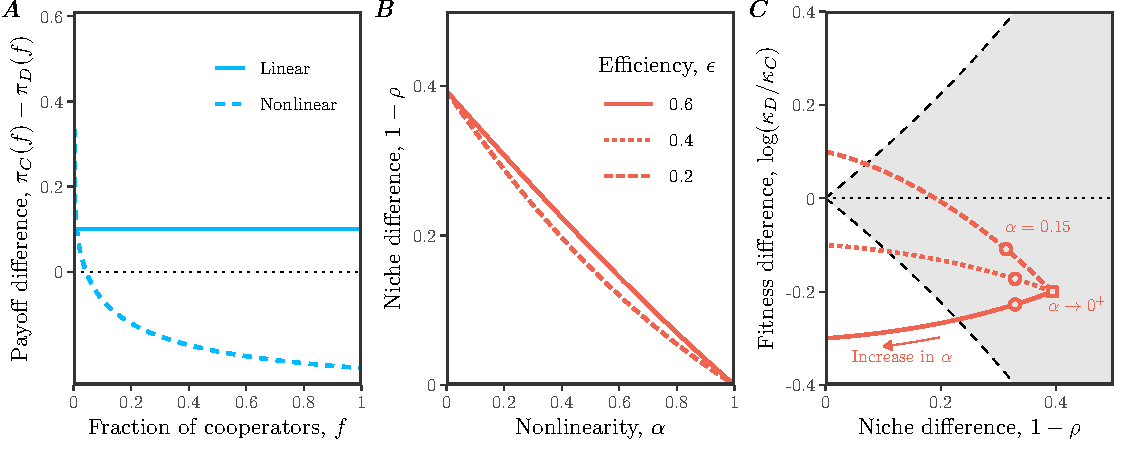
\includegraphics[width=\textwidth]{../figure/figure_microbial.pdf}
\caption{
\textbf{Effects of nonlinear microbial growth on coexistence of cooperation and defection.}
(A) Payoff differences between cooperation and defection for linear and nonlinear models of microbial growth.
In panel A, we assumed $\epsilon=0.4$, $c=0.3$, and $\alpha=0.15$ for illustrative purposes.
(B) Effect of nonlinearity $\alpha$ on niche difference $1-\rho$.
Each line assumes a different value of efficiency $\epsilon$.
Note that lines for $\epsilon=0.6$ and $\epsilon=0.4$ are nearly overlapping and are indistinguishable.
(C) Effect of nonlinearity $\alpha$ on both niche difference $1-\rho$ and fitness difference $\log(\kappa_D/\kappa_C)$.
The gray shaded area represents the coexistence regime.
The square represents the condition when $\alpha \to 0^+$.
The circles represent the condition when $\alpha=0.15$, which correspond to the experimental relationship between glucose and microbial growth \citep{gore2009snowdrift}.
In panels B and C, we assumed $c=0.3$, while allowing $\epsilon$ and $\alpha$ to vary.
}
\end{figure}

\pagebreak

\bibliography{coexistence-strategy}

\end{document}
